\documentclass[12pt]{article}

\usepackage[margin = .8in]{geometry}
\usepackage{amsmath}
\usepackage{graphicx}
\usepackage{multicol, enumerate, tabularx}
\usepackage[scaled=0.86]{helvet}

\usepackage{adjustbox}

\usepackage{fancyhdr}
\pagestyle{fancy}

\lhead{Math F113X: Numbers and Society}
\rhead{Lecture Notes}

\usepackage{tikz}
\usetikzlibrary{calc,trees,positioning,arrows,fit,shapes,through, backgrounds}
\usetikzlibrary{patterns}

\usetikzlibrary{decorations.markings}
\usetikzlibrary{arrows}

\usepackage{pgfplots}

\usepackage{longtable}
\usepackage{tabularx}

\newcommand{\ds}{\displaystyle}
\newcommand{\ans}[1][1in]{\rule{#1}{.5pt}}

\newcommand{\points}[1]{(#1 points.)}		% Trying to be lazy.

\usepackage{array}
\newcolumntype{L}[1]{>{\raggedright\let\newline\\\arraybackslash\hspace{0pt}}m{#1}}
\newcolumntype{C}[1]{>{\centering\let\newline\\\arraybackslash\hspace{0pt}}m{#1}}
\newcolumntype{R}[1]{>{\raggedleft\let\newline\\\arraybackslash\hspace{0pt}}m{#1}}
\newcommand{\red}[1]{\textcolor{red}{#1}}

\newcommand{\be}{\begin{enumerate}}
\newcommand{\ee}{\end{enumerate}}

%\topmargin -1in
%\textheight 9.5in
%\oddsidemargin -0.3in
%\evensidemargin \oddsidemargin
%\pagestyle{empty}
%%\marginparwidth 0.5in
%\textwidth 7in
%\parindent 0in

%--------------------------------------------------------------------------------------------------------------------------------------------------------------------------
%						Document
%--------------------------------------------------------------------------------------------------------------------------------------------------------------------------


\begin{document}
%\pagestyle{fancy}
\begin{center}
{\Large Hamiltonian Circuits and Paths (Day 2)}
\end{center}
%-------------------------------------------------------------------------------------------------------------
%						Assignment
%-----------------------------------------------------------------------------------------------------
\begin{enumerate}


\item Recall the problem at the end of Worksheet 14. 

\begin{quote}
Use the Nearest Neighbor Algorithm starting at vertex 0 to find a Hamiltonian circuit. Highlight the circuit on the left-hand graph.

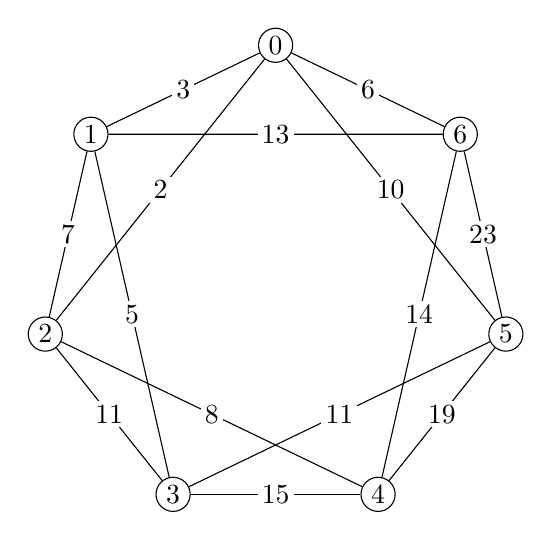
\begin{tikzpicture}[vtx/.style={draw, circle, inner sep =1.5 pt}, lbl/.style =  {inner sep =1.5 pt, fill = white}]
\foreach \i in {0,1,2,3,4,5,6}{\node[vtx] (\i) at (360*\i/7+90:3){\i};}
\foreach \i in {0,1,2,3,4,5,6}{\draw let \n1 = {int(mod(\i+1, 7))}, \n2 = {int(1*\i+3*\n1)}
 in (\i) -- node[lbl] {\n2} 
(\n1);}
\foreach \i in {0,1,2,3,4,5,6}{\draw let \n1 = {int(mod(\i+2, 7))}, \n2 = {int(2*\i+1*\n1)}
 in (\i) -- node[lbl] {\n2} 
(\n1);}
\end{tikzpicture}
\hfill
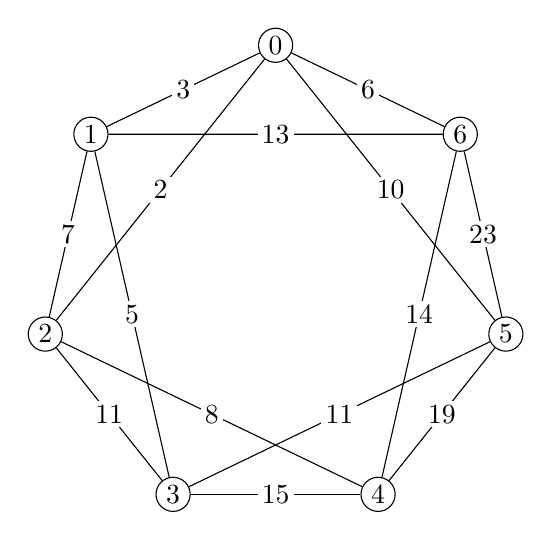
\begin{tikzpicture}[vtx/.style={draw, circle, inner sep =1.5 pt}, lbl/.style =  {inner sep =1.5 pt, fill = white}]
\foreach \i in {0,1,2,3,4,5,6}{\node[vtx] (\i) at (360*\i/7+90:3){\i};}
\foreach \i in {0,1,2,3,4,5,6}{\draw let \n1 = {int(mod(\i+1, 7))}, \n2 = {int(1*\i+3*\n1)}
 in (\i) -- node[lbl] {\n2} 
(\n1);}
\foreach \i in {0,1,2,3,4,5,6}{\draw let \n1 = {int(mod(\i+2, 7))}, \n2 = {int(2*\i+1*\n1)}
 in (\i) -- node[lbl] {\n2} 
(\n1);} 
\end{tikzpicture}
\bigskip

List the vertices of the circuit in order: \hrulefill

What is the weight of the circuit you found? \ans

The Hamiltonian circuit with smallest weight has weight 61. Can you find it? Draw it on the second graph.
\end{quote}

\item Add weights to the complete 4-vertex graph below such that NNA starting at vertex $0$ gives the \emph{highest} weight Hamiltonian circuit. (That is, show that NNA can give the worst possible answer!)\\
On the left, show the Hamiltonian circuit obtained by starting NNA at 0. On the right, find the minimum weight Hamiltonian circuit. Calculate the weights of each.

\begin{tikzpicture}[vtx/.style={draw, circle, inner sep =1.5 pt}, lbl/.style =  {inner sep =1.5 pt, fill = white}]
\foreach \i in {0,1,2,3}{\node[vtx] (\i) at (360*\i/4+90:3){\i};}
\foreach \i in {0,1,2,3}{
	\foreach \j in {0,1,2,3}{
		\draw (\i) -- (\j);}}
\end{tikzpicture}
\hfill
\begin{tikzpicture}[vtx/.style={draw, circle, inner sep =1.5 pt}, lbl/.style =  {inner sep =1.5 pt, fill = white}]
\foreach \i in {0,1,2,3}{\node[vtx] (\i) at (360*\i/4+90:3){\i};}
\foreach \i in {0,1,2,3}{
	\foreach \j in {0,1,2,3}{
		\draw (\i) -- (\j);}}
\end{tikzpicture}
\vfill
How do you \emph{know} that circuit on the right is a minimum?\\
Will NNA ever give the circuit on the right?
\newpage
\item Repeated Nearest Neighbor Algorithm: 
\vfill
\item Apply RNNA to the graph below. Break ties by choosing the smallest vertex.\\
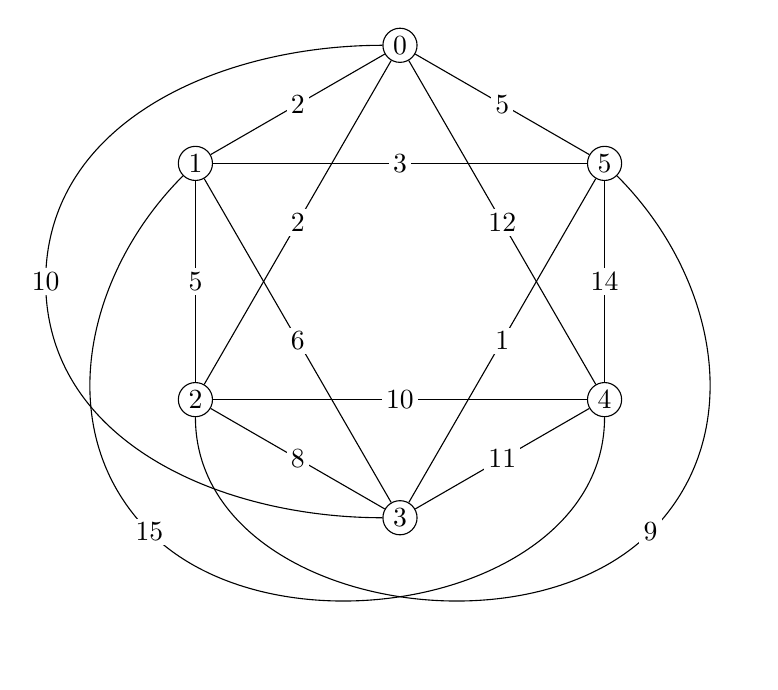
\begin{tikzpicture}[vtx/.style={draw, circle, inner sep =1.5 pt}, lbl/.style =  {inner sep =1.5 pt, fill = white}]
\foreach \i in {0,1,2,3,4,5}{\node[vtx] (\i) at (360*\i/6+90:3){\i};}
\foreach \i in {0,1,2,3,4,5}{
	\draw let \n1 = {int(mod(\i+1, 6))}, \n2 = {int(1*\i+2*\n1)} in (\i) -- node[lbl] {\n2} (\n1);
	\draw let \n3 = {int(mod(\i+2, 6))}, \n4 = {int(mod(3*\i+1*\n3,13)} in (\i) -- node[lbl] {\n4} (\n3);}
\draw (0) to [out=180,in=90] (180:4.5) to [out=270, in=180] (3);
\draw (1) to [out=225,in=135] (225:4.5) to [out=315, in=270] (4);
\draw (2) to [out=270,in=225] (315:4.5) to [out=45, in=315] (5);
\node[inner sep =1.5 pt, fill = white] at (180:4.5){$10$};
\node[inner sep =1.5 pt, fill = white] at (225:4.5){$15$};
\node[inner sep =1.5 pt, fill = white] at (315:4.5){$9$};

\end{tikzpicture}
\vfill

\vfill
\item How would be know if \emph{any} of the circuits above are optimal?
\newpage
\item Brute Force Algorithm\\
\vspace{0.5in}

\item Find a \emph{systematic} way of listing all possible circuits on four vertices with vertex set 0,1,2,3. How many are there?\\
\vspace{2in}

\item Find a \emph{systematic} way of listing all possible circuits on five vertices with vertex set 0,1,2,3,4. How many are there?\\
\vfill

\item \emph{Without} listing all possible circuits on six vertices with vertex set 0,1,2,3,4,5, how many are possible?\\
\vspace{.5in}

\item How many different circuits on 100 vertices with vertex set 0,1,2,3,4,5,...,99?\\
\vspace{.25in}
 \newpage
 \item \textbf{Factorial Notation:}
 \vfill
 
 \item \textbf{Scientific Notation:}
 \vfill
 
 \item How do you calculate $n!$ for very large $n$-values?
 
 \vfill
\end{enumerate}
\end{document}

%-------------------------------------------------------------------------------------------------------------------------------------------------------------------------------------------------------------------

%%% Local Variables:
%%% mode: latex
%%% TeX-master: t
%%% End:
